\documentclass[]{article}
\usepackage{lmodern}
\usepackage{setspace}
\setstretch{1}
\usepackage{amssymb,amsmath}
\usepackage{ifxetex,ifluatex}
\usepackage{fixltx2e} % provides \textsubscript
\ifnum 0\ifxetex 1\fi\ifluatex 1\fi=0 % if pdftex
  \usepackage[T1]{fontenc}
  \usepackage[utf8]{inputenc}
\else % if luatex or xelatex
  \ifxetex
    \usepackage{mathspec}
  \else
    \usepackage{fontspec}
  \fi
  \defaultfontfeatures{Ligatures=TeX,Scale=MatchLowercase}
\fi
% use upquote if available, for straight quotes in verbatim environments
\IfFileExists{upquote.sty}{\usepackage{upquote}}{}
% use microtype if available
\IfFileExists{microtype.sty}{%
\usepackage{microtype}
\UseMicrotypeSet[protrusion]{basicmath} % disable protrusion for tt fonts
}{}
\usepackage[margin=1in]{geometry}
\usepackage{hyperref}
\PassOptionsToPackage{usenames,dvipsnames}{color} % color is loaded by hyperref
\hypersetup{unicode=true,
            pdftitle={Component response rate variation drives stability in large complex systems},
            pdfauthor={A. Bradley Duthie},
            colorlinks=true,
            linkcolor=blue,
            citecolor=Blue,
            urlcolor=Blue,
            breaklinks=true}
\urlstyle{same}  % don't use monospace font for urls
\usepackage{graphicx,grffile}
\makeatletter
\def\maxwidth{\ifdim\Gin@nat@width>\linewidth\linewidth\else\Gin@nat@width\fi}
\def\maxheight{\ifdim\Gin@nat@height>\textheight\textheight\else\Gin@nat@height\fi}
\makeatother
% Scale images if necessary, so that they will not overflow the page
% margins by default, and it is still possible to overwrite the defaults
% using explicit options in \includegraphics[width, height, ...]{}
\setkeys{Gin}{width=\maxwidth,height=\maxheight,keepaspectratio}
\IfFileExists{parskip.sty}{%
\usepackage{parskip}
}{% else
\setlength{\parindent}{0pt}
\setlength{\parskip}{6pt plus 2pt minus 1pt}
}
\setlength{\emergencystretch}{3em}  % prevent overfull lines
\providecommand{\tightlist}{%
  \setlength{\itemsep}{0pt}\setlength{\parskip}{0pt}}
\setcounter{secnumdepth}{0}
% Redefines (sub)paragraphs to behave more like sections
\ifx\paragraph\undefined\else
\let\oldparagraph\paragraph
\renewcommand{\paragraph}[1]{\oldparagraph{#1}\mbox{}}
\fi
\ifx\subparagraph\undefined\else
\let\oldsubparagraph\subparagraph
\renewcommand{\subparagraph}[1]{\oldsubparagraph{#1}\mbox{}}
\fi

%%% Use protect on footnotes to avoid problems with footnotes in titles
\let\rmarkdownfootnote\footnote%
\def\footnote{\protect\rmarkdownfootnote}

%%% Change title format to be more compact
\usepackage{titling}

% Create subtitle command for use in maketitle
\newcommand{\subtitle}[1]{
  \posttitle{
    \begin{center}\large#1\end{center}
    }
}

\setlength{\droptitle}{-2em}
  \title{Component response rate variation drives stability in large complex
systems}
  \pretitle{\vspace{\droptitle}\centering\huge}
  \posttitle{\par}
  \author{A. Bradley Duthie}
  \preauthor{\centering\large\emph}
  \postauthor{\par}
  \predate{\centering\large\emph}
  \postdate{\par}
  \date{Biological and Environmental Sciences, University of Stirling, Stirling,
UK, FK9 4LA
\href{mailto:alexander.duthie@stir.ac.uk}{\nolinkurl{alexander.duthie@stir.ac.uk}}}

\usepackage{amsmath}
\usepackage{natbib}
\usepackage{lineno}
\usepackage[utf8]{inputenc}
\linenumbers
\bibliographystyle{amnatnat}

\begin{document}
\maketitle

\begin{center}\rule{0.5\linewidth}{\linethickness}\end{center}

\textbf{The stability of a complex system generally decreases with
increasing system size, as is demonstrated by random matrix
theory\textsuperscript{\protect\hyperlink{ref-May1972}{1},\protect\hyperlink{ref-Allesina2012}{2}}.
This counter-intuitive result, first shown by
May\textsuperscript{\protect\hyperlink{ref-May1972}{1}}, is broadly
relevant for understanding the dynamics and persistence of systems such
as
ecological\textsuperscript{\protect\hyperlink{ref-May1972}{1},\protect\hyperlink{ref-Allesina2012}{2}},
neurological\textsuperscript{\protect\hyperlink{ref-Gray2008}{3},\protect\hyperlink{ref-Gray2009}{4}},
biochemical\textsuperscript{\protect\hyperlink{ref-Rosenfeld2009}{5},\protect\hyperlink{ref-MacArthur2010}{6}}
and
socio-economic\textsuperscript{\protect\hyperlink{ref-Haldane2011}{7}--\protect\hyperlink{ref-Bardoscia2017}{9}}
networks. Much attention has especially been given to the stability of
ecological communities such as food webs or mutualist networks, with
recent work investigating how different community structures affect
stability\textsuperscript{\protect\hyperlink{ref-Allesina2012}{2},\protect\hyperlink{ref-Mougi2012}{10}--\protect\hyperlink{ref-Patel2018}{14}}.
But more broadly, stabilising mechanisms in complex systems remain
under-developed, and the effect of variation in the response rate of
individual system components remains an open
problem\textsuperscript{\protect\hyperlink{ref-Allesina2015}{15}}. Here
I show that when components of a complex system respond to system
dynamics at different rates (\(\boldsymbol{\gamma}\)), the potential for
system stability is markedly increased. Stability is caused by the
clustering of some eigenvalues toward the centre of eigenvalue
distributions despite the destabilising effect of higher interaction
strength variation (\(\boldsymbol{\sigma^{2}}\)). This effect of
variation in \(\boldsymbol{\gamma}\) becomes increasingly important as
system size increases, to the extent that the largest stable complex
systems would otherwise be unstable if not for
\(\boldsymbol{Var(\gamma)}\). My results therefore reveal a previously
unconsidered driver of system stability that is likely to be pervasive
across all complex systems. Future research in complex systems should
therefore account for the varying response rates of individual system
components when assessing whole system stability.}

In 1972, May\textsuperscript{\protect\hyperlink{ref-May1972}{1}} first
demonstrated that randomly assembled systems of sufficient complexity
are almost inevitably unstable given infinitesimally small
perturbations. Complexity in this case is defined by the size of the
system (i.e., the number of interacting components; \(S\)), its
inter-connectivity (i.e., the probability that one component will affect
another; \(C\)), and the variance of interaction strengths
(\(\sigma^{2}\))\textsuperscript{\protect\hyperlink{ref-Allesina2012}{2}}.
May's finding that the probability of local stability falls to near zero
given a sufficiently high threshold of \(\sigma\sqrt{SC}\) has profound
consequences across multiple disciplines, raising the question of how
complex systems in, e.g.,
ecology\textsuperscript{\protect\hyperlink{ref-Allesina2012}{2},\protect\hyperlink{ref-Mougi2012}{10},\protect\hyperlink{ref-Grilli2017}{13},\protect\hyperlink{ref-Allesina2015}{15}}
or
banking\textsuperscript{\protect\hyperlink{ref-Haldane2011}{7},\protect\hyperlink{ref-Bardoscia2017}{9},\protect\hyperlink{ref-May2008}{16}}
are predicted to persist or change.

Randomly assembled complex systems can be represented as large square
matrices (\(M\)) with \(S\) components (e.g.,
species\textsuperscript{\protect\hyperlink{ref-Allesina2012}{2}} or
banks\textsuperscript{\protect\hyperlink{ref-Haldane2011}{7}}). One
element of such a matrix \(M_{ij}\) defines how component \(j\) affects
component \(i\) in the system at a point of
equilibrium\textsuperscript{\protect\hyperlink{ref-Allesina2012}{2}}.
Off-diagonal elements (\(i \neq j\)) therefore define interactions
between components, while diagonal elements (\(i = j\)) define component
self-regulation (e.g., carrying capacity in ecological communities).
Traditionally, values of off-diagonal elements are assigned non-zero
values with a probability \(C\), which are sampled from a distribution
with variance \(\sigma^{2}\); diagonal elements are set to
-1\textsuperscript{\protect\hyperlink{ref-May1972}{1},\protect\hyperlink{ref-Allesina2012}{2},\protect\hyperlink{ref-Allesina2015}{15}}.
Local system stability is assessed using eigenanalysis, with the system
being stable if the real parts of all eigenvalues (\(\lambda\)) of \(M\)
are negative
(\(\max\left(\Re(\lambda)\right) < 0\))\textsuperscript{\protect\hyperlink{ref-May1972}{1},\protect\hyperlink{ref-Allesina2012}{2}}.
In a large system (high \(S\)), eigenvalues are distributed
uniformly\textsuperscript{\protect\hyperlink{ref-Tao2010}{17}} within a
circle centred at \(\Re = -1\) (the mean value of diagonal elements) and
\(\Im = 0\), with a radius of
\(\sigma\sqrt{SC}\)\textsuperscript{\protect\hyperlink{ref-May1972}{1},\protect\hyperlink{ref-Allesina2012}{2},\protect\hyperlink{ref-Allesina2015}{15}}
(Figs 1a and 2a). Local stability of randomly assembled systems
therefore becomes increasingly unlikely as \(S\), \(C\), and
\(\sigma^{2}\) increase.

The above stability criterion assumes that individual components respond
to perturbations of the system at the same rate (\(\gamma\)), but this
is highly unlikely in any complex system. In ecological communities, for
example, the rate at which population density changes following
perturbation will depend on the generation time of individuals, which
might vary by orders of magnitude among species. Species with short
generation times will respond quickly (high \(\gamma\)) to perturbations
relative to species with long generation times (low \(\gamma\)).
Similarly, the speed at which individual banks respond to perturbations
in financial networks, or individuals or institutions respond to
perturbations in complex social networks, is likely to vary. The effect
of such variance has not been investigated in complex systems theory.
Intuitively, variation in \(\gamma\) might be expected to decrease
system stability by introducing a new source of variation into the
system and thereby increasing \(\sigma\). Here I show why, despite
higher \(\sigma\), complex systems in which \(\gamma\) varies are
actually more likely to be stable, especially when \(S\) is high.

\begin{center}\rule{0.5\linewidth}{\linethickness}\end{center}

\textbf{Figure 1: Example distribution of eigenvalues before (a) and
after (b) separating a randomly generated complex system into fast
(\(\boldsymbol{\gamma} = 1.95\)) and slow
(\(\boldsymbol{\gamma} = 0.05\)) component response rates.} Each panel
shows the same system where \(S = 200\), \(C = 0.05\), and
\(\sigma = 0.4\), and in each case \(E[\gamma] = 1\) (i.e., only the
distribution of \(\gamma\) differs between panels). \textbf{a.}
Eigenvalues plotted when all \(\gamma = 1\); distributions of points are
uniformly distributed within the grey circle with a radius of
\(\sigma\sqrt{SC} =\) 1.238 centred at -1 on the real axis. \textbf{b.}
Eigenvalues plotted when half \(\gamma = 1.95\) and half
\(\gamma = 0.05\); distributions of points can be partitioned into one
large circle of \(\sigma\sqrt{SC} =\) 1.718 centred at
\(\gamma = -1.95\) and one small circle of \(\sigma\sqrt{SC} =\) 0.044
centred at \(\gamma = -0.05\). In a, the maximum real eigenvalaue
\(\max\left(\Re(\lambda)\right) =\) 0.2344871, while in b
\(\max\left(\Re(\lambda)\right) =\) -0.0002273135, meaning that the
complex system in b but not a is stable because in b
\(\max\left(\Re(\lambda)\right) < 0\). In 1 million randomly generated
complex systems under the same parameter values, 1 was stable when
\(\gamma = 1\) while 32 were stable when \(\gamma = \{1.95, 0.05\}\).
Overall, complex systems that are separated into fast versus slow
components tend to be more stable than otherwise identical systems with
identical component response rates.

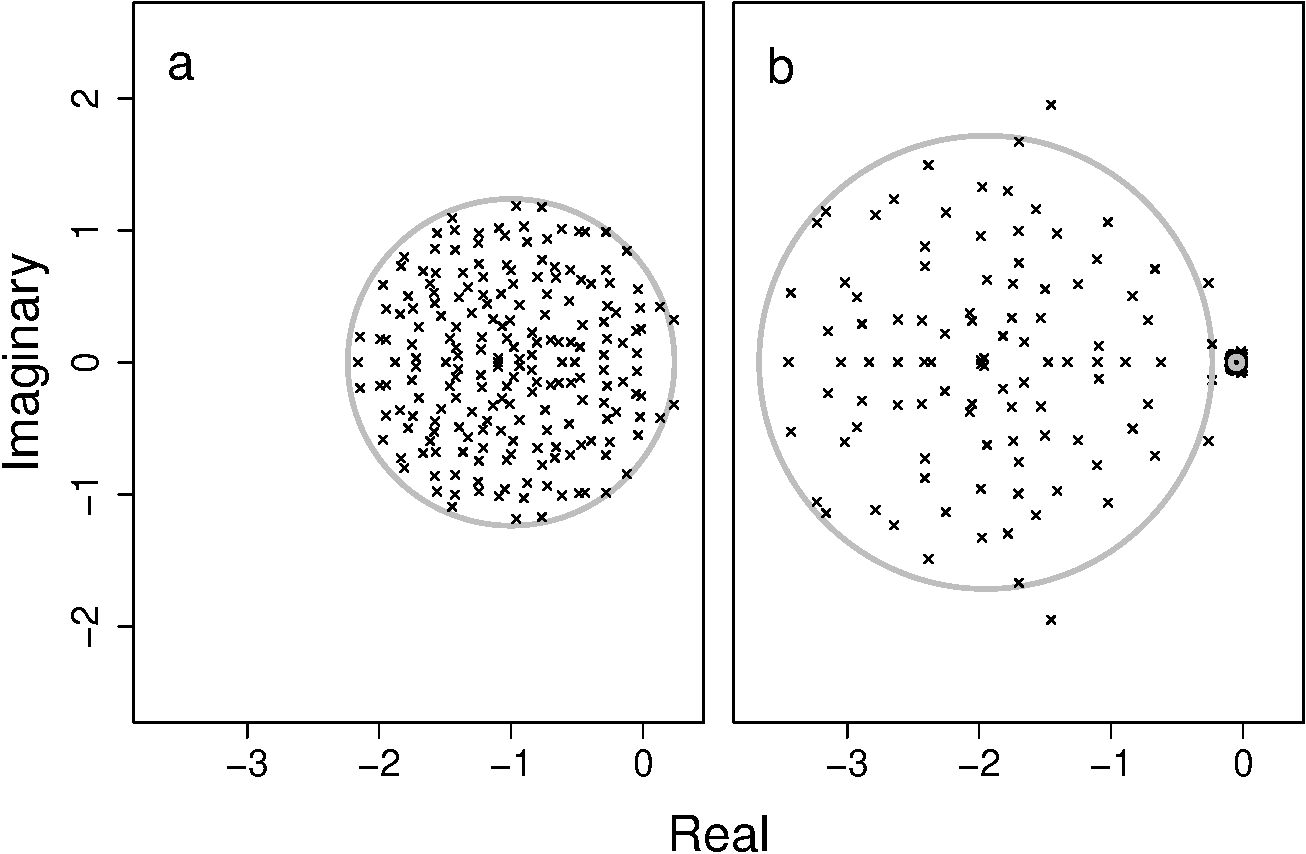
\includegraphics{ms_files/figure-latex/unnamed-chunk-4-1.pdf}

\begin{center}\rule{0.5\linewidth}{\linethickness}\end{center}

Rows in \(M\) define how a given component \(i\) is affected by other
components of the system, meaning that the rate of component response
time can be modelled by multiplying all row elements by a real scalar
value
\(\gamma_{i}\)\textsuperscript{\protect\hyperlink{ref-Patel2018}{14}}.
The distribution of \(\gamma\) over \(S\) components thereby models the
distribution of component response rates. An instructive example
compares one \(M\) where \(\gamma_{i} = 1\) for all \(i\) in \(S\) to
the same \(M\) when half of \(\gamma_{i} = 1.95\) and half of
\(\gamma_{i} = 0.05\). This models one system in which \(\gamma\) is
invariant and one in which \(\gamma\) varies, but systems are otherwise
identical (note \(E[\gamma_{i}] = 1\) in both cases). I assume
\(S = 200\), \(C = 0.05\), and \(\sigma = 0.4\); diagonal elements are
set to \(-1\) and non-zero off-diagonal elements are drawn from
\(\mathcal{N}(0, \sigma^{2})\). Rows are then multiplied by
\(\gamma_{i}\) to generate \(M\). When \(\gamma_{i} = 1\), eigenvalues
of \(M\) are distributed uniformly within a circle centred at
(\(-1, 0\)) with a radius of 1.265 (Fig. 1a). Hence, the real components
of eigenvalues are highly unlikely to all be negative when all
\(\gamma_{i} = 1\). But when \(\gamma_{i}\) values are separated into
two groups, eigenvalues are no longer uniformly distributed (Fig. 1b).
Instead, two distinct clusters of eigenvalues appear (grey circles in
Fig. 1b), one centred at (\(-1.95, 0\)) and the other centred at
(\(-0.05, 0\)). The former has a large radius, but the real components
have shifted to the left (in comparison to when \(\gamma = 1\)) and all
\(\Re({\lambda}) < 0\). The latter cluster has real components that have
shifted to the right, but has a smaller radius. Overall, for 1 million
randomly assembled \(M\), this division between slow and fast component
response rates results in more stable systems: 1 stable given
\(\gamma = 1\) versus 32 stable given \(\gamma = \{1.95, 0.5\}\).

\begin{center}\rule{0.5\linewidth}{\linethickness}\end{center}

\textbf{Figure 2: Distributions of eigenvalues before (a) and after (b)
introducing variation in component response rate
(\(\boldsymbol{\gamma}\)) in complex systems.} Each panel show the same
system where \(S = 1000\), \(C = 1\), and \(\sigma = 0.4\). \textbf{a.}
Eigenvalues plotted in the absence of \(Var(\gamma)\) where
\(E[\gamma] = 1\), versus \textbf{b.} eigenvalues plotted given
\(\gamma \sim \mathcal{U}(0, 2)\), which increases the variance of
interaction strengths (\(\sigma^{2}\)) but clusters eigenvalues toward
the distribution's centre (-1, 0). Black and red elipses in both panels
show the circle centred on the distribution in panels a and b,
respectively, which have a radius of \(\sigma \sqrt{SC}\). Proportions
of \(\Re(\lambda) < 0\) are 0.551 and 0.553 for a and b, respectively.

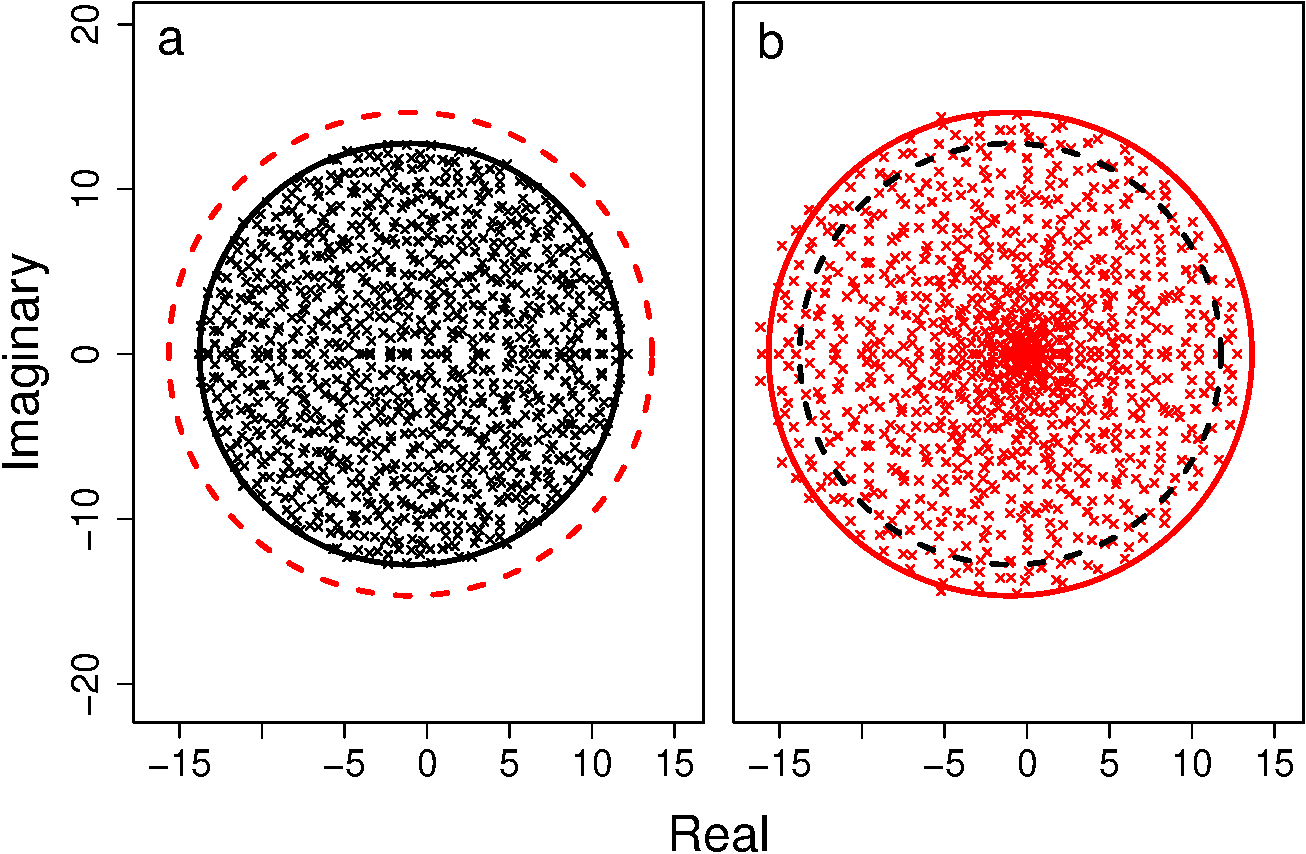
\includegraphics{ms_files/figure-latex/unnamed-chunk-7-1.pdf}

\begin{center}\rule{0.5\linewidth}{\linethickness}\end{center}

Higher stability in systems with variation in \(\gamma\) can be observed
by sampling \(\gamma_{i}\) values from various distributions. I now
focus on a uniform distribution where \(\gamma \sim \mathcal{U}(0, 2)\)
(see Supplementary Information for other distributions, which give
similar results). As with the case of \(\gamma = \{1.95, 0.5\}\) (Fig.
1b), \(E[\gamma] = 1\) when \(\gamma \sim \mathcal{U}(0, 2)\), allowing
comparison of \(M\) before and after variation in component response
rate. Figure 2 shows a comparison of eigenvalue distributions given
\(S = 1000\), \(C = 1\), and \(\sigma = 0.4\). As
expected\textsuperscript{\protect\hyperlink{ref-Tao2010}{17}}, when
\(\gamma = 1\), eigenvalues are distributed uniformly in a circle
centred at (\(-1, 0\)) with a radius of \(\sigma\sqrt{SC} =\) 12.649.
Uniform variation in \(\gamma\) leads to a non-uniform distribution of
eigenvalues, some of which are clustered tightly around the centre of
the distribution, but others of which are spread outside the former
radius of 12.649 (red circle Fig 2b). This larger radius occurs because
the addition of \(Var(\gamma)\) increases the realised \(\sigma\) of
\(M\). The clustering and spreading of eigenvalues introduced by
\(Var(\gamma)\) can destabilise previously stable systems or stabilise
systems that are otherwise unstable. But where systems are otherwise too
complex to be stable given \(\gamma = 1\), the effect of \(Var(\gamma)\)
can often lead to stability above
May's\textsuperscript{\protect\hyperlink{ref-May1972}{1},\protect\hyperlink{ref-Allesina2012}{2}}
threshold of \(\sigma\sqrt{SC} > 1\).

\begin{center}\rule{0.5\linewidth}{\linethickness}\end{center}

\textbf{Figure 3: Stability of large complex systems with and without
variation in component response rate(\(\boldsymbol{\gamma}\)).} The
\(\ln\) number of systems that are stable across different system sizes
(\(S\)) given \(C = 1\), and the proportion of systems in which
variation in \(\gamma\) is critical for system stability. For each
\(S\), 1 million complex systems are randomly generated. Stability of
each complex system is tested given variation in \(\gamma\) by randomly
sampling \(\gamma \sim \mathcal{U}(0, 2)\). Stability given
\(Var(\gamma)\) is then compared to stability in an otherwise identical
system in which \(\gamma = E[\mathcal{U}(0, 2)]\) for all components.
Light and dark grey bars show the number of stable systems in the
absence and presence of \(Var(\gamma)\), respectively. The black line
shows the proportion of systems that are stable when
\(Var(\gamma) > 0\), but would be unstable if \(Var(\gamma) = 0\).

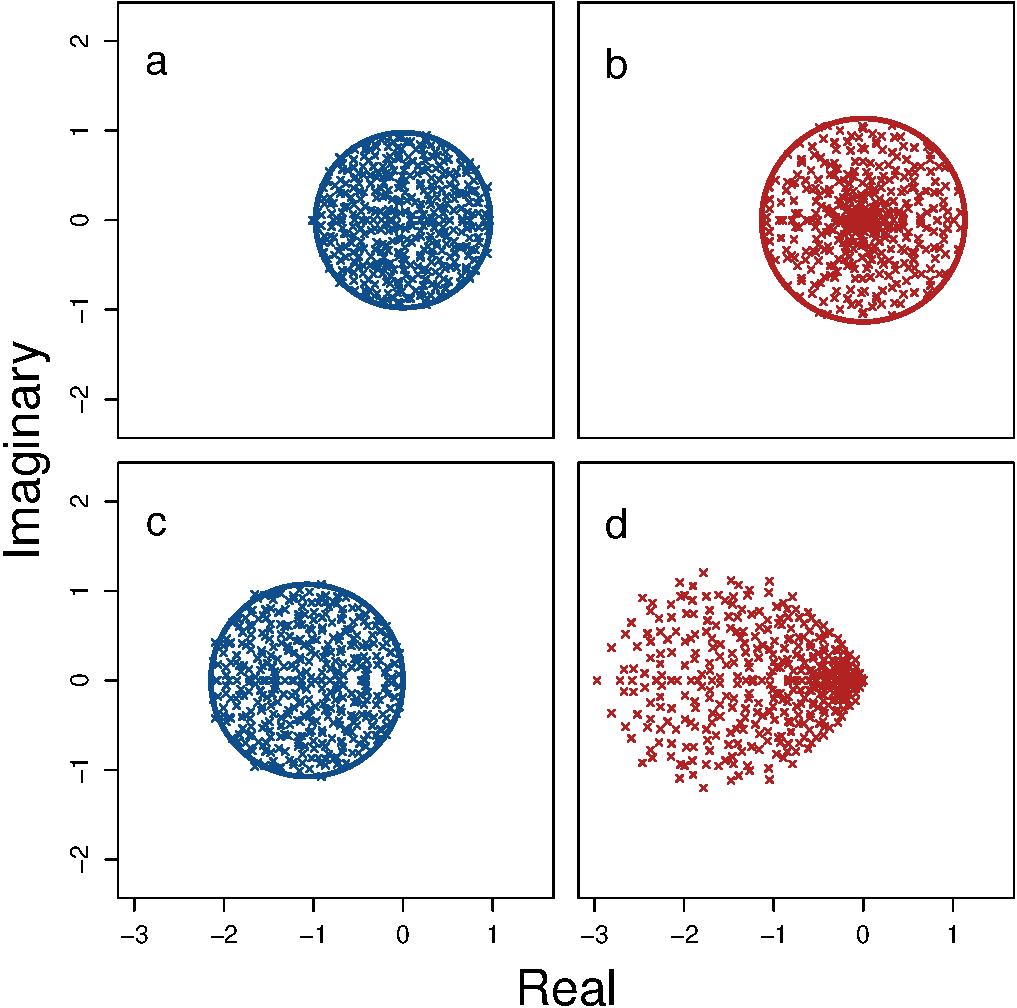
\includegraphics{ms_files/figure-latex/unnamed-chunk-9-1.pdf}

\begin{center}\rule{0.5\linewidth}{\linethickness}\end{center}

To investigate the effect of \(Var(\gamma)\) on system stability, I
simulated random \(M\) matrices at \(\sigma = 0.4\) and \(C = 1\) across
\(S\) ranging from \(2-32\) (see Supplementary Information for different
values of \(\sigma\) and \(C\)). One million \(M\) were simulated for
each \(S\), and the stability of \(M\) was assessed given \(\gamma = 1\)
versus \(\gamma \sim \mathcal{U}(0, 2)\) (note that under these
conditions, \(\sigma\sqrt{SC} = 1\) given \(S = 25\) when
\(\gamma = 1\)). I found that the number of stable random systems was
consistently higher given \(Var(\gamma)\) than when \(\gamma = 1\) (Fig.
3), and that the difference between the probabilities of observing a
stable system increased with an increase in \(S\); i.e., the potential
for \(Var(\gamma)\) to drive stability increased with system complexity.
For the highest values of \(S\), nearly all systems that were stable
given \(Var(\gamma)\) would not have been stable given \(\gamma = 1\),
and the maximum observed \(S\) for which a system was stable was \(31\)
given \(Var(\gamma)\) versus \(27\) given \(\gamma = 1\) (see
Supplementary Information for full results). This suggests that the
stability of large systems might be dependent upon variation in the
response rate of their individual components, meaning that factors such
as generation time (in ecological networks), transaction speed (in
economic networks), or communication speed (in social networks) needs to
be considered when investigating the stability of complex systems.

Some care is needed when interpreting these results. First, I emphasise
that \(Var(\gamma)\) is not stabilising per se; that is, adding
variation in \(\gamma\) to a particular system \(M\) does not
necessarily increase the probability that the system will be stable (see
Supplementary Information). Rather, systems that are observed to be
stable are more likely to vary in \(\gamma\), and for this
\(Var(\gamma)\) to be critical to their stability. This is caused by the
shift in the distribution of eigenvalues that occurs by introducing
\(Var(\gamma)\) (Fig. 1b, 2b), which can sometimes result in all
\(\Re(\lambda) < 0\) but might also increase \(\Re(\lambda)\) values. To
further investigate the potential of \(Var(\gamma)\) to be stabilising,
I used a simple genetic algorithm (the space of possible \(\gamma\)
values was too large to searh
exhaustively\textsuperscript{\protect\hyperlink{ref-Hamblin2013}{18}};
see Supplementary Information). For each of 10000 random \(M\), the
genetic algorithm initialised 1000 different sets of
\(\gamma \sim \mathcal{U}(0, 2)\) values of size \(S\). Eigenanalysis of
each set of \(\gamma\) values was performed, and the 20 sets with the
lowest \(\max\left(\Re(\lambda)\right)\) each produced 50 offspring with
subsequent mutation and crossover between the resulting new population
of 1000 \(\gamma\) sets. The genetic algorithm terminated if a stable
\(M\) was found, 20 generations occurred, or a converge criteria of
minimum fitness increase between generations was satisfied. Across
\(S = \{2, 3, ..., 39, 40\}\), sets of \(\gamma\) values were frequently
found that resulted in stable systems (the highest at \(S = 39\)),
suggesting that varying component response time might by itself be
sufficient to stabilise complex systems.

I have focused broadly on random complex systems, but it is also
worthwhile to consider more restricted interactions such as those of
specific ecological
networks\textsuperscript{\protect\hyperlink{ref-Allesina2012}{2}}. These
include systems in which all interactions (i.e., all off-diagonal
elements of \(M\)) are negative (e.g., competitive networks), positive
(e.g., mutualist networks), or \(i\) and \(j\) pairs have opposing signs
(e.g., predator-prey networks). In general, competitive and mutualist
networks tend to be destabilising, and predator-prey network tend to be
stabilising\textsuperscript{\protect\hyperlink{ref-Allesina2011}{19}}.
When \(Var(\gamma)\) is applied to each, the proportion of stable
competitive and predator-prey networks increases, but the proportion of
stable mutualist communities does not (see Supplementary Information).
Additionally, when each component of \(M\) is interpreted as a unique
species and given a random intrinsic growth
rate\textsuperscript{\protect\hyperlink{ref-Dougoud2018}{20}},
feasibility is not increased by \(Var(\gamma)\), suggesting that
variation in species generation time might be unlikely to drive
stability in purely multi-species networks (see Supplementary
Information).

My results show that complex systems are more likely to be stable when
the response rates of system components vary. These results are broadly
applicable to complex biological and social networks.

\begin{center}\rule{0.5\linewidth}{\linethickness}\end{center}

\textbf{References}

\hypertarget{refs}{}
\hypertarget{ref-May1972}{}
1. May, R. M. Will a large complex system be stable? \emph{Nature}
\textbf{238,} 413--414 (1972).

\hypertarget{ref-Allesina2012}{}
2. Allesina, S. \& Tang, S. Stability criteria for complex ecosystems.
\emph{Nature} \textbf{483,} 205--208 (2012).

\hypertarget{ref-Gray2008}{}
3. Gray, R. T. \& Robinson, P. A. Stability and synchronization of
random brain networks with a distribution of connection strengths.
\emph{Neurocomputing} \textbf{71,} 1373--1387 (2008).

\hypertarget{ref-Gray2009}{}
4. Gray, R. T. \& Robinson, P. A. Stability of random brain networks
with excitatory and inhibitory connections. \emph{Neurocomputing}
\textbf{72,} 1849--1858 (2009).

\hypertarget{ref-Rosenfeld2009}{}
5. Rosenfeld, S. Patterns of stochastic behavior in dynamically unstable
high-dimensional biochemical networks. \emph{Gene Regulation and Systems
Biology} \textbf{3,} 1--10 (2009).

\hypertarget{ref-MacArthur2010}{}
6. MacArthur, B. D., Sanchez-Garcia, R. J. \& Ma'ayan, A. Microdynamics
and criticality of adaptive regulatory networks. \emph{Physics Review
Letters} \textbf{104,} 168701 (2010).

\hypertarget{ref-Haldane2011}{}
7. Haldane, A. G. \& May, R. M. Systemic risk in banking ecosystems.
\emph{Nature} \textbf{469,} 351--355 (2011).

\hypertarget{ref-Suweis2014}{}
8. Suweis, S. \& D'Odorico, P. Early warning signs in social-ecological
networks. \emph{PLoS ONE} \textbf{9,} (2014).

\hypertarget{ref-Bardoscia2017}{}
9. Bardoscia, M., Battiston, S., Caccioli, F. \& Caldarelli, G. Pathways
towards instability in financial networks. \emph{Nature Communications}
\textbf{8,} 1--7 (2017).

\hypertarget{ref-Mougi2012}{}
10. Mougi, A. \& Kondoh, M. Diversity of interaction types and
ecological community stability. \emph{Science} \textbf{337,} 349--351
(2012).

\hypertarget{ref-Allesina2015a}{}
11. Allesina, S. \& Tang, S. The stability--complexity relationship at
age 40: a random matrix perspective. \emph{Population Ecology} 63--75
(2015).
doi:\href{https://doi.org/10.1007/s10144-014-0471-0}{10.1007/s10144-014-0471-0}

\hypertarget{ref-Gao2016}{}
12. Gao, J., Barzel, B. \& Barabási, A. L. Universal resilience patterns
in complex networks. \emph{Nature} \textbf{530,} 307--312 (2016).

\hypertarget{ref-Grilli2017}{}
13. Grilli, J. \emph{et al.} Feasibility and coexistence of large
ecological communities. \emph{Nature Communications} \textbf{8,} (2017).

\hypertarget{ref-Patel2018}{}
14. Patel, S., Cortez, M. H. \& Schreiber, S. J. Partitioning the
effects of eco-evolutionary feedbacks on community stability.
\emph{American Naturalist} \textbf{191,} 1--29 (2018).

\hypertarget{ref-Allesina2015}{}
15. Allesina, S. \emph{et al.} Predicting the stability of large
structured food webs. \emph{Nature Communications} \textbf{6,} 7842
(2015).

\hypertarget{ref-May2008}{}
16. May, R. M., Levin, S. A. \& Sugihara, G. Complex systems: Ecology
for bankers. \emph{Nature} \textbf{451,} 893--895 (2008).

\hypertarget{ref-Tao2010}{}
17. Tao, T. \& Vu, V. Random matrices: Universality of ESDs and the
circular law. \emph{Annals of Probability} \textbf{38,} 2023--2065
(2010).

\hypertarget{ref-Hamblin2013}{}
18. Hamblin, S. On the practical usage of genetic algorithms in ecology
and evolution. \emph{Methods in Ecology and Evolution} \textbf{4,}
184--194 (2013).

\hypertarget{ref-Allesina2011}{}
19. Allesina, S. \& Levine, J. M. A competitive network theory of
species diversity. \emph{Proceedings of the National Academy of Sciences
of the United States of America} \textbf{108,} 5638--5642 (2011).

\hypertarget{ref-Dougoud2018}{}
20. Dougoud, M., Vinckenbosch, L., Rohr, R., Bersier, L.-F. \& Mazza, C.
The feasibility of equilibria in large ecosystems: a primary but
neglected concept in the complexity-stability debate. \emph{PLOS
Computational Biology} \textbf{14,} e1005988 (2018).


\end{document}
